\documentclass[11pt,spanish]{article}

\usepackage{listings}
\usepackage{anysize} 
\usepackage{graphicx}
\usepackage[spanish]{babel}
\usepackage[utf8]{inputenc}
\usepackage{xcolor}
\usepackage{wrapfig}


\lstset{language=Python}
\marginsize{1cm}{1cm}{2cm}{2cm}
\selectlanguage{spanish}
\lstset{
language=Python,
 backgroundcolor=\color{red!75!green!50!blue!25},
 frame=single,
literate=
  {á}{{\'a}}1 {é}{{\'e}}1 {í}{{\'i}}1 {ó}{{\'o}}1 {ú}{{\'u}}1
  {Á}{{\'A}}1 {É}{{\'E}}1 {Í}{{\'I}}1 {Ó}{{\'O}}1 {Ú}{{\'U}}1
  {à}{{\`a}}1 {è}{{\`e}}1 {ì}{{\`i}}1 {ò}{{\`o}}1 {ù}{{\`u}}1
  {À}{{\`A}}1 {È}{{\'E}}1 {Ì}{{\`I}}1 {Ò}{{\`O}}1 {Ù}{{\`U}}1
  {ä}{{\"a}}1 {ë}{{\"e}}1 {ï}{{\"i}}1 {ö}{{\"o}}1 {ü}{{\"u}}1
  {Ä}{{\"A}}1 {Ë}{{\"E}}1 {Ï}{{\"I}}1 {Ö}{{\"O}}1 {Ü}{{\"U}}1
  {â}{{\^a}}1 {ê}{{\^e}}1 {î}{{\^i}}1 {ô}{{\^o}}1 {û}{{\^u}}1
  {Â}{{\^A}}1 {Ê}{{\^E}}1 {Î}{{\^I}}1 {Ô}{{\^O}}1 {Û}{{\^U}}1
  {œ}{{\oe}}1 {Œ}{{\OE}}1 {æ}{{\ae}}1 {Æ}{{\AE}}1 {ß}{{\ss}}1
  {ű}{{\H{u}}}1 {Ű}{{\H{U}}}1 {ő}{{\H{o}}}1 {Ő}{{\H{O}}}1
  {ç}{{\c c}}1 {Ç}{{\c C}}1 {ø}{{\o}}1 {å}{{\r a}}1 {Å}{{\r A}}1
  {€}{{\EUR}}1 {£}{{\pounds}}1
}


\title{\vspace{-3cm}\begin{flushleft}\textbf{Actividad 3}\end{flushleft}}
\author{\hspace{-9.6cm}\textsc{Andrés Ignacio Rodríguez Mendoza}}
\date{}

\begin{document}

\begin{wrapfigure}{r}{0.2\textwidth}
  \begin{center}
   \vspace{-5.4cm} 
\includegraphics[width=0.15\textwidth]{uni}
  \end{center}
\end{wrapfigure}

\maketitle  
\begin{center}
\rule{\textwidth}{1pt}
\end{center}

$$\alpha$$

\section*{Código}

\begin{lstlisting} % Start your code-block

import numpy as np
import matplotlib.pyplot as plt
from scipy.interpolate import interp1d


#    Dados 10 puntos aleatorios entre x=0 y x=3 para la función f(x) = sin(2 x).
x0 = 3*np.random.random(10)
y0 = np.sin(2*x0)

#    Dados 20 puntos aleatorios entre x=-10 y x=10 para la función f(x) = sin(x)/x
x1 = 20*np.random.random(20) -10
y1 = np.sin(x1)/x1

#    Dados 16 puntos aleatorios entre x=-3 y x=3 para la función f(x) = x^2sin(2x)
x2 = 6*np.random.random(16) - 3
y2 = x2*x2 *np.sin(2*x2)

#    Dados 12 puntos aleatorios entre x=-2 y x=2 para la función f(x) = x^3sin(3x)
x3 = 4*np.random.random(12) -2
y3 =  x3*x3*x3*np.sin(3*x3)

# Array with points in between those of the data set for interpolation.
x_0 = np.linspace(min(x0),max(x0),100)
x_1 = np.linspace(min(x1),max(x1),100)
x_2 = np.linspace(min(x2),max(x2),100)
x_3 = np.linspace(min(x3),max(x3),100)

# Available options for interp1d
options = ('linear','quadratic','cubic')



#plot 1
plt.plot(x0, y0, 'o', label='Data')
for o in options:
    f = interp1d(x0, y0, kind=o)   
    plt.plot(x_0, f(x_0), label=o)      
plt.title('f(x) = sin(2 x)')
plt.legend()
plt.show()

#plot2
plt.plot(x1, y1, 'o', label='Data1')
for o in options:
    f = interp1d(x1, y1, kind=o)    
    plt.plot(x_1, f(x_1), label=o)     
plt.title('f(x) = sin(x)/x')
plt.legend()
plt.show()
#plot3
plt.plot(x2, y2, 'o', label='Data2')
for o in options:
    f = interp1d(x2, y2, kind=o)    
    plt.plot(x_2, f(x_2), label=o)    
plt.title('f(x) = x^2 sin(2 x)')
plt.legend()
plt.show()

#plot4
plt.plot(x3, y3, 'o', label='Data3')
for o in options:
    f = interp1d(x3, y3, kind=o)    
    plt.plot(x_3, f(x_3), label=o)     
plt.title('f(x) = x^3 sin(3 x)')
plt.legend()
plt.show()

\end{lstlisting}


\section*{Gŕaficas}

\centering 

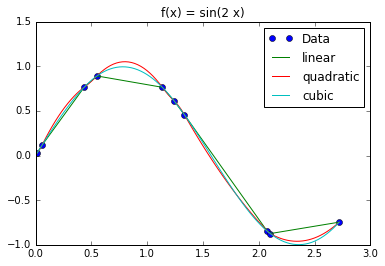
\includegraphics{1}\\
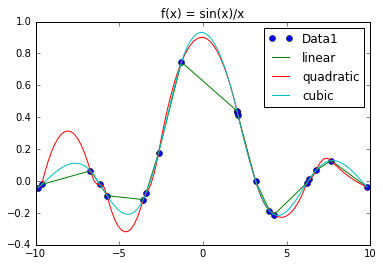
\includegraphics{2}\\
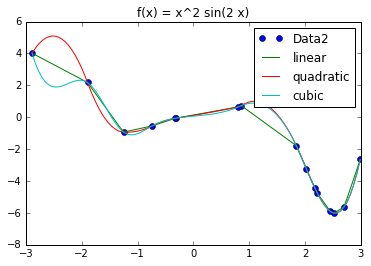
\includegraphics{3}\\
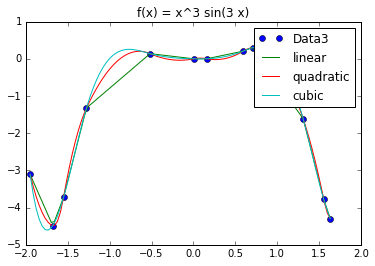
\includegraphics{4}\\





\end{document}

